\chapter{The HSR Problem and The State-of-the-art Algorithms}

This chapter describes the HSR problem in detail.
The organization of this chapter is as follows.
First the HS and MS sensor characteristics are discussed, followed by the
signal model that simulates their characteristics are developed.
Then we described the commonly used signal model for hyperspectral images
named "Linear Mixing Model" (LMM).
Finally the HSR problem statement is presented.

%The HSR problem statement is a hyperspectral unmixing (HU) based MF problem
%that finds an estimate of the underlying endmember signatures and
%their corresponding abundance, which constitute the desired SR image, from
%the HS and MS image pair.

\section{Signal Model of HS and MS Sensors}
Let $\bm{\mathcal Y} \in \R_+^{\ell_1 \times \ell_2 \times M}$ be a
nonnegative tensor representing the pixel values of an SR image with
$L = \ell_1 \cdot \ell_2$ pixels and with $M$ spectral bands.
The tensor $\bm{\mathcal Y}$ can be lexicographically unfolded to a
nonnegative matrix $\bm Y \in \R_+^{M \times L}$.
The column-wise view and row-wise view of $\bm Y$ are shown in
\eqref{eq:col_view_Y} and \eqref{eq:row_view_Y}, respectively, such that
$\{\bm y_i\}_{i=1}^L \in \R_+^M$ represents the spectral reflectance signature
at the $i\thtxt$ pixel and $\{\bm y^j\}_{j=1}^M \in \R_+^L$ represents the
%vectorized abundance fraction map of all endmembers at the $j\thtxt$
vectorized reflectance map of the SR image at the $j\thtxt$
spectral band.
Figure \ref{fig:HSI_unfolding} illustrates the process of unfolding a spectral
image from a tensor to a matrix.
\begin{eqnarray}
    \bm Y & = & \begin{bmatrix} \bm y_1 & \bm y_2 & \cdots & \bm y_L \end{bmatrix} \label{eq:col_view_Y} \\
    \bm Y & = & \begin{bmatrix} \bm y^1 & \bm y^2 & \cdots & \bm y^M \end{bmatrix}^\text T
    \label{eq:row_view_Y}
\end{eqnarray}

\begin{figure}[t]
    \centering
    \resizebox{0.85\linewidth}{!}{
        \begin{tikzpicture}
            \node at (0,0)   [xshift=   0cm,yshift=   0cm]                                (center) {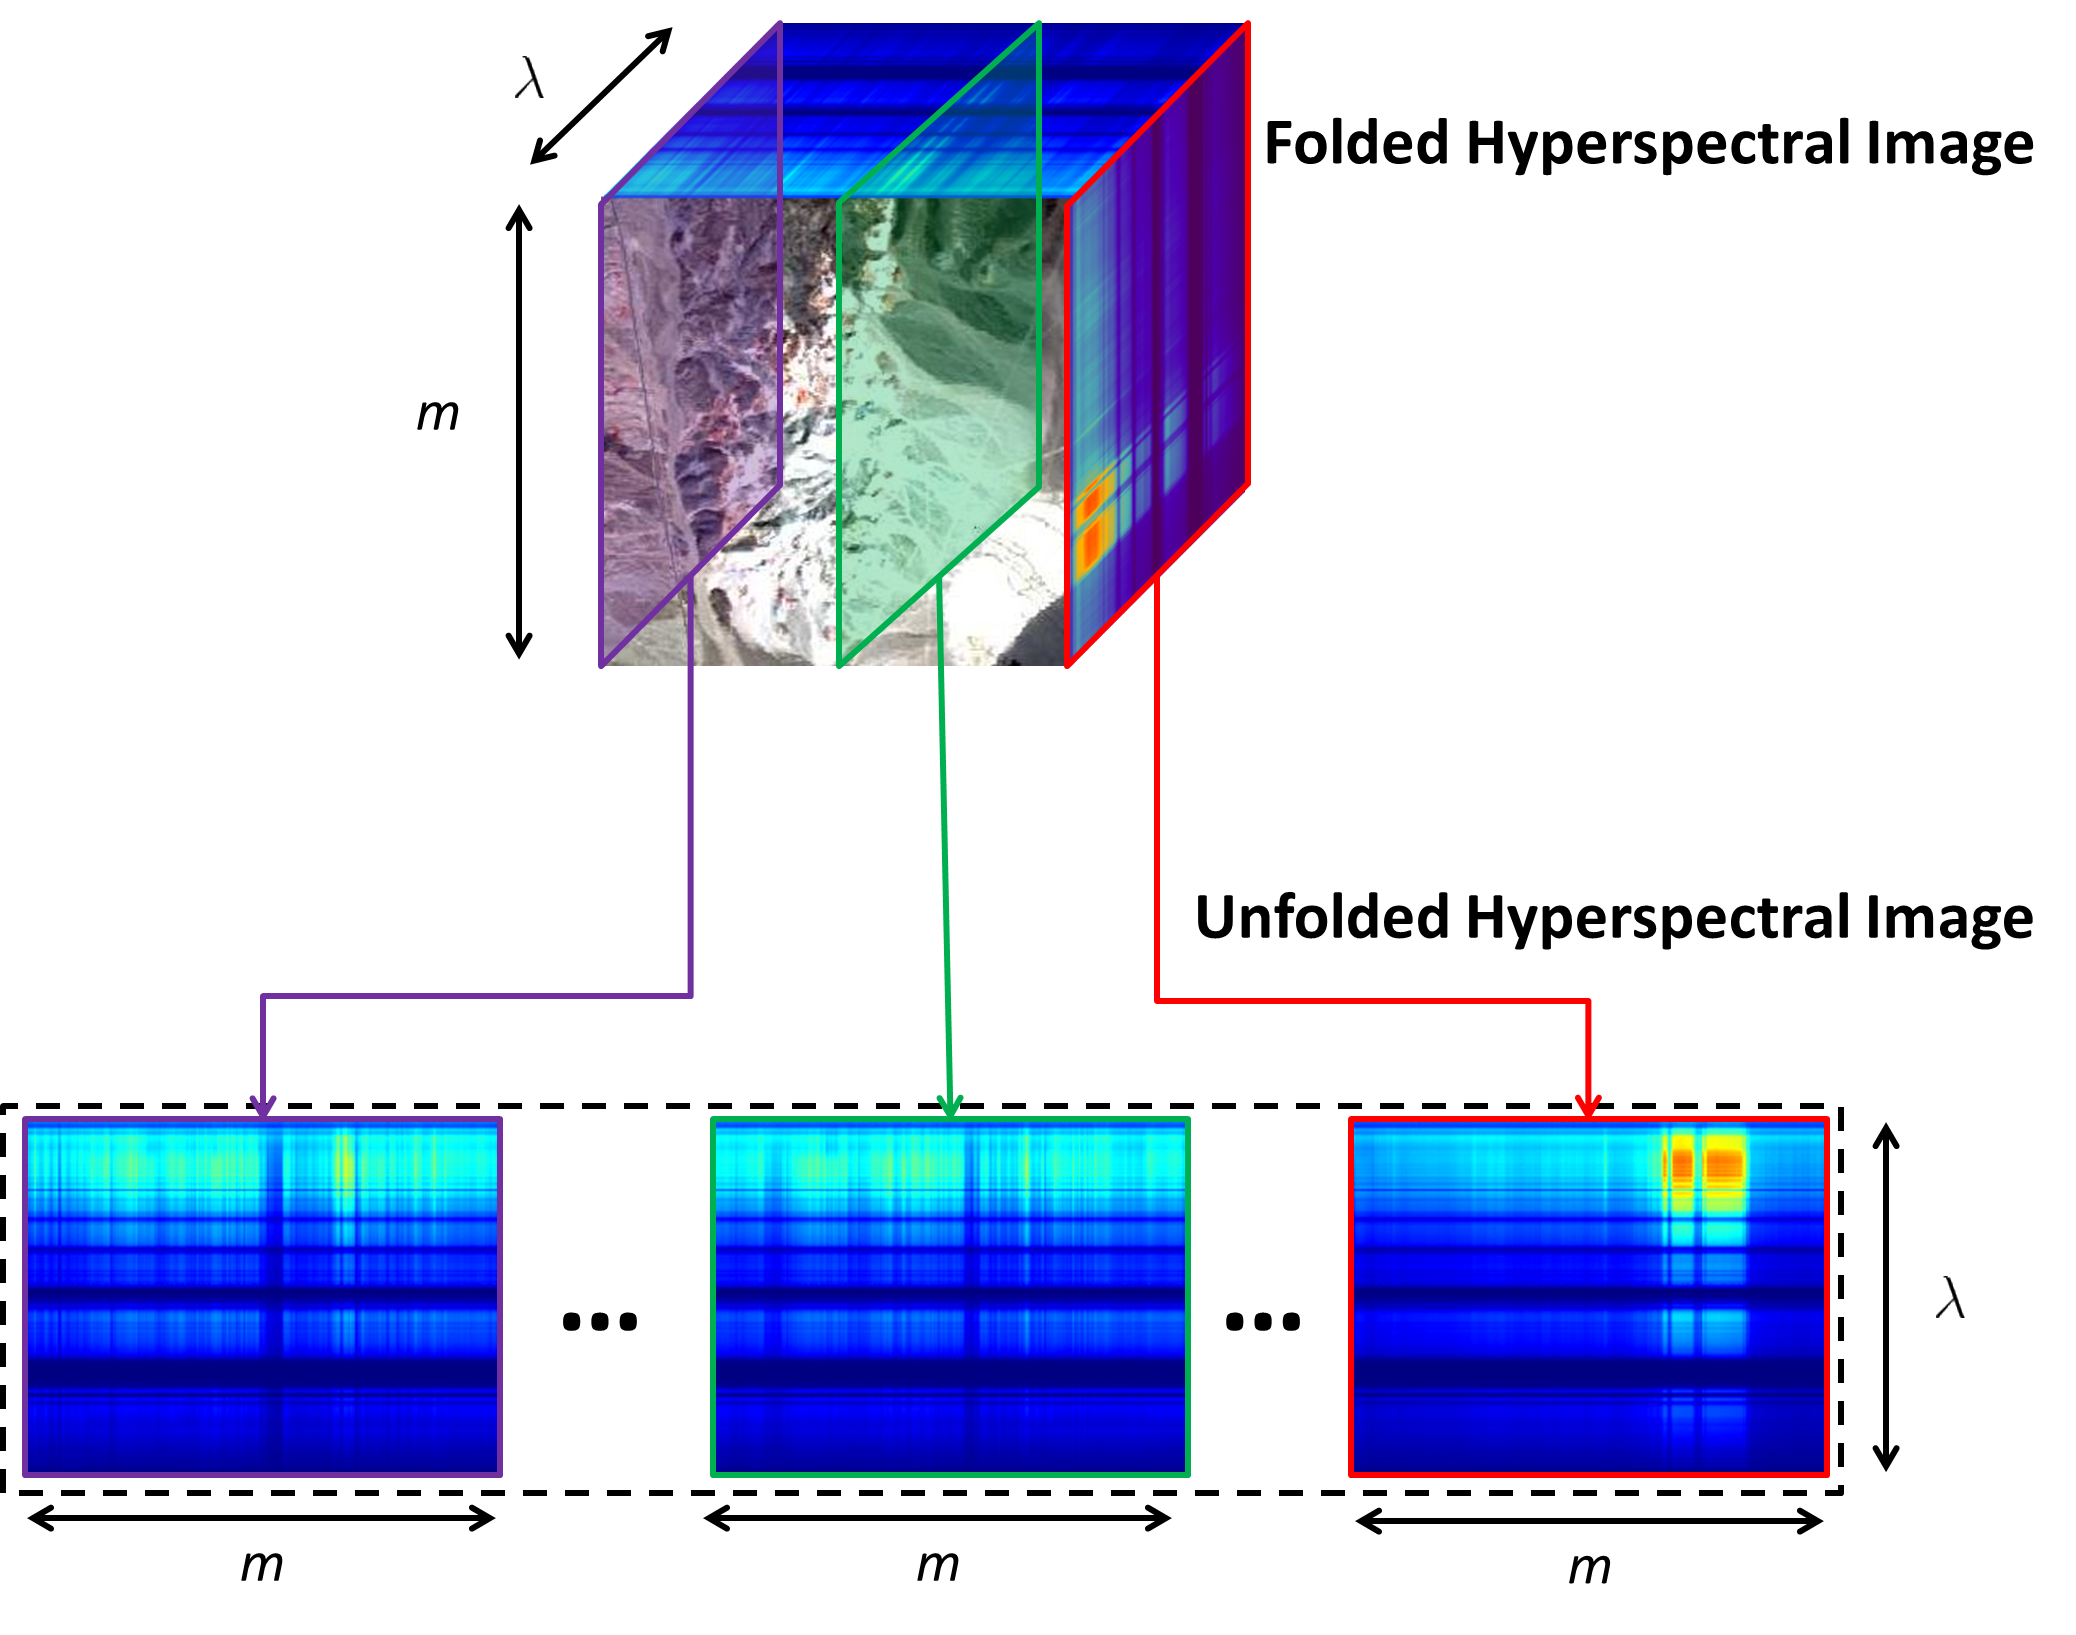
\includegraphics[width=0.8\columnwidth]{./fig/fig_02HSR_Problem/HSR_Problem_HSI_unfolding}} ;
            \node at (center)[xshift= 3.9cm,yshift= 3.8cm,text width=5cm  ,fill=white!20]          {Folded Hyperspectral Image};
            \node at (center)[xshift= 3.9cm,yshift=-0.5cm,text width=6cm  ,fill=white!20]          {Unfolded Hyperspectral Image};
            \node at (center)[xshift=-3.5cm,yshift= 2.2cm,text width=0.5cm,fill=white!20]          {$\ell_1$};
            \node at (center)[xshift=-4.3cm,yshift=-4.4cm,text width=0.5cm,fill=white!20] (t1)     {$\ell_1$};
            \node at (t1)    [xshift= 3.8cm,yshift=   0cm,text width=0.5cm,fill=white!20] (t2)     {$\ell_1$};
            \node at (t2)    [xshift= 3.8cm,yshift=   0cm,text width=0.5cm,fill=white!20]          {$\ell_1$};
            \node at (center)[xshift=-3.1cm,yshift= 4.1cm,text width=0.5cm,fill=white!20]          {$M$};
            \node at (center)[xshift= 5.3cm,yshift=-2.8cm,text width=0.5cm,fill=white!20]          {$M$};
        \end{tikzpicture}
    }
    \caption{Unfolding a hyperspectral image from a tensor to a matrix.}
    \label{fig:HSI_unfolding}
\end{figure}

In the signal model an SR image is partially observed by an HS sensor and by
an MS sensor.
Let $\YH\in\R_+^{M \times L_\text H}$ and $\YM\in\R_+^{M_\text M \times L}$
represent the vectorized observed HS and MS images, respectively, where
$L_\text H$ is the number of pixels of the HS image and $M_\text M$ is the
number of spectral bands of the MS image.
As introduced in Section \ref{sec:HSR}, we know that HS images have higher
spectral resolution and MS images have higher spatial resolution so that the
following inequality hold:
\begin{eqnarray}
    M         & > & M_\text M, \\
    L_\text H & < & L.
\end{eqnarray}
\begin{figure}[t]
    \centering
    \subfigure[$\;$]{\label{fig:IMG_DOWNSAMP_full400x400}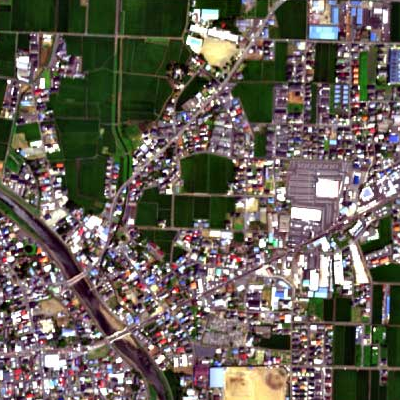
\includegraphics[width=0.3\columnwidth]{./fig/fig_02HSR_Problem/IMG_DOWNSAMP_full400x400}}
    \subfigure[$\;$]{\label{fig:IMG_DOWNSAMP_blur400x400}
\includegraphics[width=0.3\columnwidth]{./fig/fig_02HSR_Problem/IMG_DOWNSAMP_blur400x400}}
    \subfigure[$\;$]{\label{fig:IMG_DOWNSAMP_down50x50}  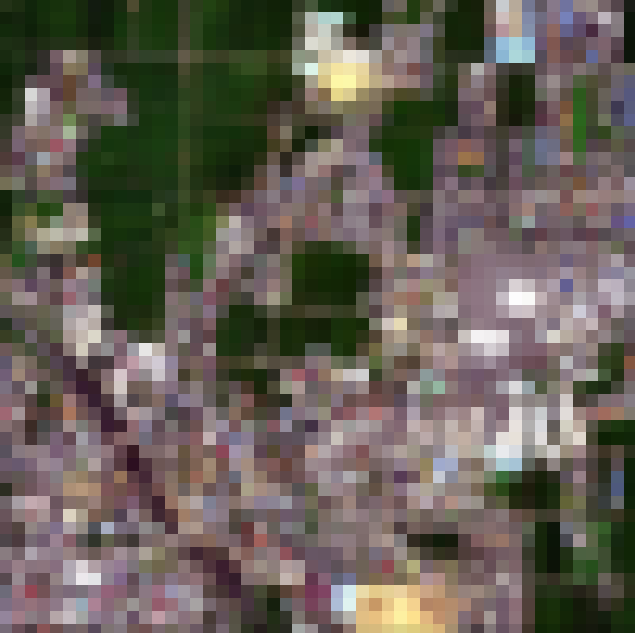
\includegraphics[width=0.3\columnwidth]{./fig/fig_02HSR_Problem/IMG_DOWNSAMP_down50x50}  }
    \caption{Effect of spatial degradation by HS sensors:
             (a) High spatial resolution image with $400 \times 400$ pixels;
             (b) Image of (a) blurred by a $25 \times 25$ Gaussian filter of
                 variance $\sigma = 3$;
             (c) Image of (b) subsampled on every $8$ pixels vertically and
                 horizontally.}
    \label{fig:IMG_DOWNSAMP_down80x80}
\end{figure}

\subsection{Spatial Degradation Model in HS Sensors}\label{sec:SPATIAL_DOWNSAMPL_MODEL}
An HS sensor degrades the spatial contents of SR images.
The relation between $\bm Y$ and $\YH$ can be modelled as
\begin{equation}
    \YH = \bm Y \bm G + \bm V_\text H,
    \label{eq:spatial_degradation_model}
\end{equation}
where $\bm G \in \R^{L \times L_\text H}$ is a matrix representing the spatial
degradation effect that may be composed of geometric wrapping, translation,
blurring and subsampling operations and $\bm V_\text H$ represents the noise
in the HS sensor.
Note that $\bm G$ is a matrix multiplied to the vectorized reflectance maps of
each band $\{(\bm y^j)\Tr\}_{j=1}^N$.
In this thesis the spatial responses considered include blurring and
subsampling operations.
Therefore, $\bm G$ can be expressed as
\begin{equation}
    \bm G = \bm B \bm D,
    \label{eq:spatial_degradation_model_G}
\end{equation}
where the multiplication with $\bm B \in \R^{L \times L}$ and
$\bm D \in \R^{L \times L_\text H}$ represents two different stages of spatial
responses.
The first stage is a spatial low-pass filtering where the $\ell\thtxt$ column
of $\bm B$ is a vectorized point spread function applied onto the $\ell\thtxt$
pixel of $\bm Y$.
Typically $\bm B = [\bm b_1 \cdots \bm b_L]$ is a convolution matrix of a two
dimensional normalized low-pass filter kernel.
The second stage is a spatial subsampling process with
$\bm D \in \{0,1\}^{L \times L_\text H}$ being a subsampling matrix that draws
the reflectance maps $\{(\bm y^j)\Tr\}_{j=1}^M$ vertically and horizontally on
every $d$ pixels, where $d = \sqrt{L/L_\text H}$ is the downsampling
factor.
Figure \ref{fig:IMG_DOWNSAMP_down80x80} illustrates a standard high spatial
resolution color image (a), passing through a spatial low-pass filter
(b), and then further passing through a subsampling response (c).

\subsection{Spectral Degradation Model in MS Sensors}\label{sec:SPECTRAL_DOWNSAMPL_MODEL}
An MS sensor undersamples the SR images in spectral domain by receiving signals
at fewer but wider spectral range, resulting in MS images having only few
broad band images.
The matrices $\bm Y$ and $\YM$ can be related by
\begin{equation}
    \YM = \bm F \bm Y + \bm V_\text M,
    \label{eq:spectral_degradation_model}
\end{equation}
where $\bm F \in \R_+^{M_\text M \times M}$ represents the spectral degradation
matrix of the MS sensor system; $\bm V_\text M$ is the noise in the MS sensor.

To better illustrate the spectral response of HS and MS sensors, we take an
airborne hyperspectral sensor named "AVIRIS" and a satellite multispectral
sensor named "Thematic Mapper (TM) Sensor" as examples.
They have been serving as the core instruments of NASA's Earth monitoring
projects for many years since mid 80s.
The AVIRIS sensor, as introduced in Chapter 1, observes the Earth surface at
$224$ spectral bands covering wavelengths between $0.4\,\mu$m and $2.5\,\mu$m
at norminally $10\,$nm intervals.
The TM sensor, on the other hand, observes the Earth surface at fewer spectral
bands with a wider interval.
Among them, six of which overlap with the spectral range of the AVIRIS sensor
($0.4\,\mu$m-$2.5\,\mu$m).
The spectral response of the TM sensor is shown in Figure
\ref{fig:LANDSAT7_TM_RSR}
\cite{LANDSAT_SPECTRAL_RESPONSE,
      LANDSAT_HANDBOOK,
      SPECTRAL_RESPONSE_OF_LANDSAT8}.
\begin{figure}[t]
    \centering
    \resizebox{0.98\linewidth}{!}{
        \begin{tikzpicture}
            % HS Matrix
            \node at (0,0) [xshift=0cm,yshift=0cm] (nRSR) {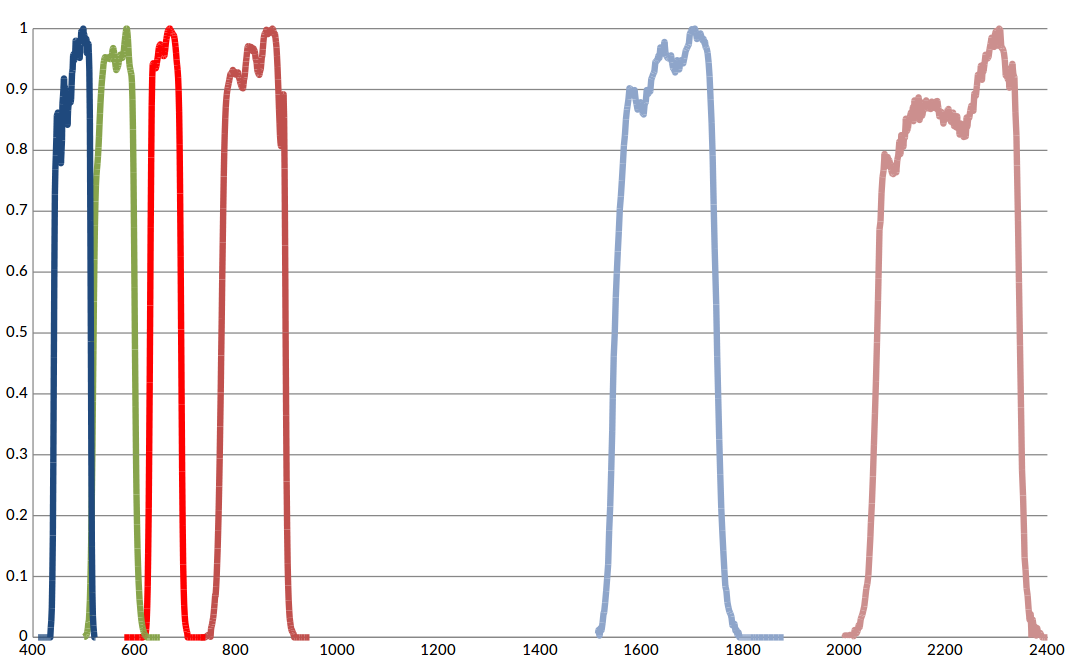
\includegraphics[width=15cm]{./fig/fig_02HSR_Problem/LANDSAT7_MS_RSR}};
            %\node at (nRSR)[xshift=0cm,yshift=6cm] (ntitle) {\Large \textbf{Relative Spectral Response of the Operational TM Sensor in LANDSAT 7 Project}} ;
            \node at (nRSR)[xshift=-8cm,rotate=90] (nylabel) {Spectral Response} ;
            \node at (nRSR)[xshift=0cm,yshift=-5cm] (nxlabel) {Wavelength (nm)} ;
        \end{tikzpicture}
    }
    \caption{Spectral response of the operational TM sensor in
             LANDSAT 7 Project
             \cite{LANDSAT_SPECTRAL_RESPONSE,
                   LANDSAT_HANDBOOK,
                   SPECTRAL_RESPONSE_OF_LANDSAT8}.}
    \label{fig:LANDSAT7_TM_RSR}
\end{figure}
The comparison of spectral characteristics between AVIRIS and TM sensors are
shown in table \ref{table:spectral_characteristics_AVIRIS_TM}.
We can see that a single spectral band of the TM sensor covers multiple
number of AVIRIS spectral bands.
\begin{table}[t]
    \centering
    \begin{tabular}{|c|c|c|l|}
        \hline
        Wavelength ($\mu\,m$) & TM Band & AVIRIS Band & Spectral Band Placement      \\ \hline
        $0.45 - 0.52$         & $1$     & $10 - 16$   & Visible (VIS-B)              \\
        $0.52 - 0.60$         & $2$     & $17 - 24$   & Visible (VIS-G)              \\
        $0.63 - 0.69$         & $3$     & $28 - 35$   & Visible (VIS-R)              \\
        $0.76 - 0.90$         & $4$     & $44 - 57$   & Near Infrared (NIR)          \\
        $1.55 - 1.75$         & $5$     & $127 - 146$ & Short Wave Infrared (SWIR-1) \\
        $10.4 - 12.5$         & $6$     & $-$         & Thermal Infrared (TIR)       \\
        $2.08 - 2.35$         & $7$     & $180 - 208$ & Short Wave Infrared (SWIR-2) \\ \hline
    \end{tabular}
    \caption{Spectral characteristics of TM sensor and AVIRIS sensor
             \cite{AVIRIS,
                   LANDSAT_USING,
                   LANDSAT_HANDBOOK,
                   MILITARY_UTILITY,
                   SPECTRAL_RESPONSE_OF_LANDSAT8}.}
    \label{table:spectral_characteristics_AVIRIS_TM}
\end{table}

\section{Low-Rank Representation of HSIs: the Linear Mixing Model (LMM)}
In the literature, the geoscience and remote sensing community have long
believed HSIs to be high dimensional data with low-rank characteristics
\cite{INTERPRET_RESIDUAL_IMG_SPECTRAL_MIXTURE_ANALYSIS_OF_AVIRIS_IMG,
      BLIND_HU_BY_EXTENDED_LMM,
      CONSTRAINED_SUBPIXEL_TARGET_DETECT_FOR_HSI,
      CONVEX_FORMULATION_HSR_VIA_SUBSPACE_REGULAR,
      DENOIS_HSI_BY_LOWRANK_REPRESENT,
      DISTRIBUT_BLIND_HU_VIA_JOINT_SPARS_LOWRANK_NMF,
      FULLY_CONSTRAINED_LS_LINEAR_SPECTRAL_MIXTURE_ANALYSIS,
      FUMI,
      FUSE,
      HALS_RANK2NMF,
      HSI_RESOTRE_LOWRANK_REPRESENT_SPECTRAL_DIFF_IMG,
      HSI_RESTORE_LOWRANK_MATRIX_RECOVER,
      HSR_BY_JOINTCRITERION_NMF,
      HYSIME,
      JOINT_HSR_AND_HU_INTERACTIVE_FEEDBACK,
      LINEAR_SPECTRAL_RANDOM_MIXTURE_ANALYSIS_FOR_HSI,
      LOWRANK_SUBSPACE_REPRESENT_ESTIMATE_NO_OF_SIGNAL_HSI,
      MVES,
      SNNMF}.
From the low-rank model of HSIs, hyperspectral imagery techniques have been
successfully devised based on the Linear Mixing Model (LMM) \eqref{eq:LMM}
which assumes that the spectral signatures in the HSIs are linearly mixed
\cite{INTERPRET_RESIDUAL_IMG_SPECTRAL_MIXTURE_ANALYSIS_OF_AVIRIS_IMG,
      BLIND_HU_BY_EXTENDED_LMM,
      CNMF,
      CONSTRAINED_SUBPIXEL_TARGET_DETECT_FOR_HSI,
      CONVEX_FORMULATION_HSR_VIA_SUBSPACE_REGULAR,
      DENOIS_HSI_BY_LOWRANK_REPRESENT,
      DISTRIBUT_BLIND_HU_VIA_JOINT_SPARS_LOWRANK_NMF,
      FULLY_CONSTRAINED_LS_LINEAR_SPECTRAL_MIXTURE_ANALYSIS,
      FUMI,
      FUSE,
      HALS_RANK2NMF,
      HSR_BY_JOINTCRITERION_NMF,
      HYSIME,
      ICE,
      JOINT_HSR_AND_HU_INTERACTIVE_FEEDBACK,
      LINEAR_SPECTRAL_RANDOM_MIXTURE_ANALYSIS_FOR_HSI,
      LOWRANK_SUBSPACE_REPRESENT_ESTIMATE_NO_OF_SIGNAL_HSI,
      MVCNMF,
      MVES,
      RVM,
      SISAL,
      SNNMF,
      VCA}.
Specifically, a HSI matrix can be expressed as
\begin{subequations}
    \begin{eqnarray}
        \bm Y & = & \begin{bmatrix} \bm y_1 & \cdots & \bm y_L \end{bmatrix} \\
              & = & \begin{bmatrix} \bm a_1 & \cdots & \bm a_N \end{bmatrix}
                    \begin{bmatrix} \bm s_1 & \cdots & \bm s_L \end{bmatrix} \\
              & = & \begin{bmatrix} \displaystyle \sum_{n=1}^N \bm a_n s_{n,1} & \cdots & \displaystyle \sum_{n=1}^N \bm a_n s_{n,L} \end{bmatrix} \\
              & = & \bm A \bm S,
    \end{eqnarray}
    \label{eq:LMM}
\end{subequations}
where $N$, also called the "model order", is the total number of material in
$\bm Y$; $\bm A \in \R^{M \times N}$ is the endmember matrix that is tall and
contains those $N$ distinct material spectra $\{\bm a_i\}_{i=1}^N$ in the HSI;
$\{\bm s_j\}_{j=1}^L$ is the $N$-dimensional abundance vector at the $j\thtxt$
pixel such that the fat abundance matrix $\bm S \in \R^{N \times L}$ tells the
contribution of the distinct material spectra in the image.
Usually $N$ is assumed to be small, \ie $N \ll \min \{M,L\}$.

Despite the popularity of the LMM model, it is not always true when the acquired HSI
exhibits linearity.
As discussed in
\cite{SPECTRAL_UNMIXING},
LMM is more likely to be valid if the endmembers in a pixel appear in
spatially segregated patterns (Figure \ref{fig:LMM_HOLDS}), while is less
likely to be valid if light is multiply scattered before reaching the sensor
(Figure \ref{fig:LMM_DOESNTHOLD}).
\begin{figure}[t]
    \centering
    \subfigure[$\;$]{\label{fig:LMM_HOLDS}     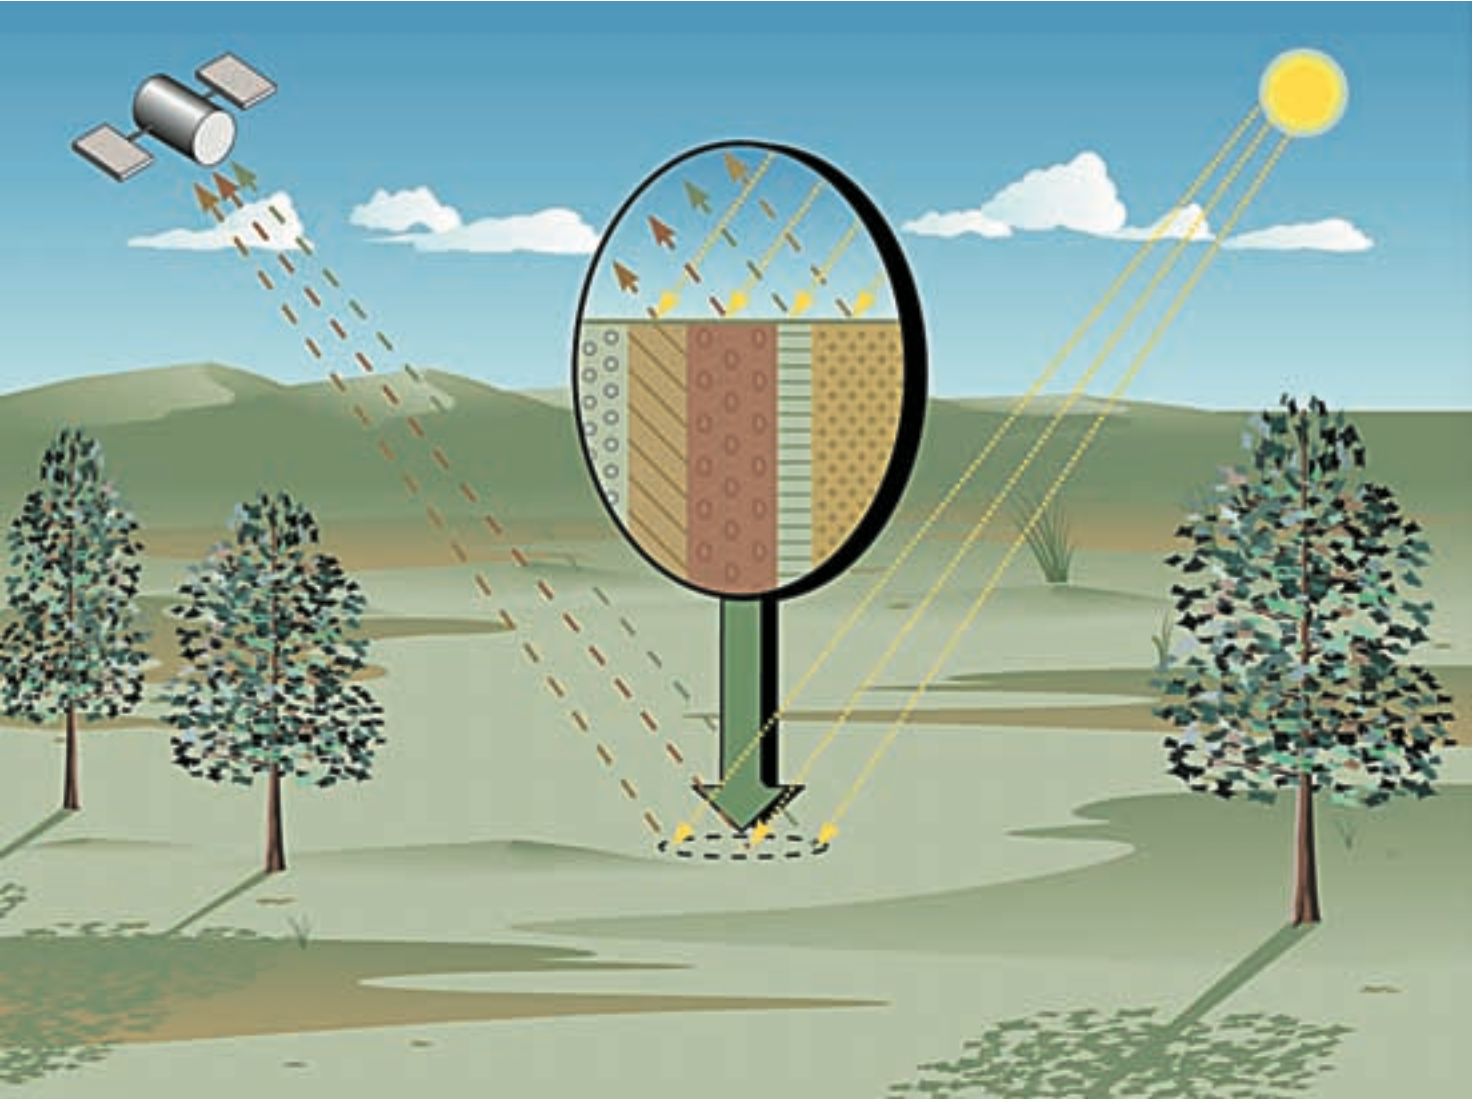
\includegraphics[width=0.48\columnwidth]{./fig/fig_02HSR_Problem/LMM_holds}}
    \subfigure[$\;$]{\label{fig:LMM_DOESNTHOLD}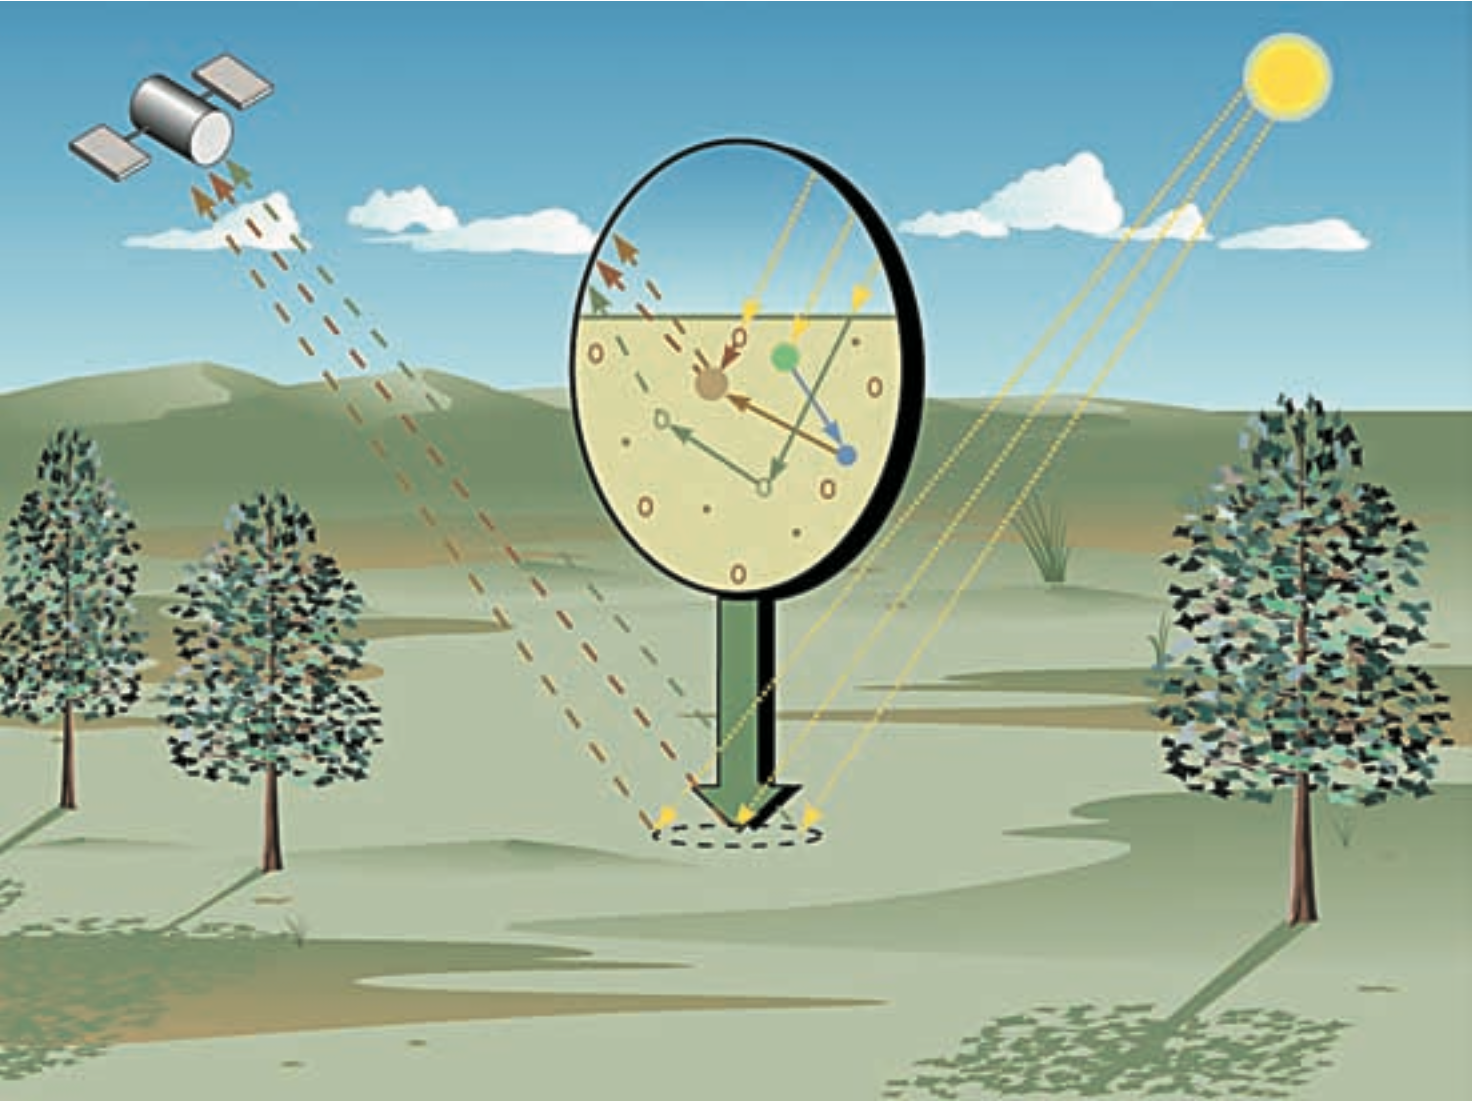
\includegraphics[width=0.48\columnwidth]{./fig/fig_02HSR_Problem/LMM_doesnthold}}
    \caption{Scenarios when LMM is (a) more likely to hold; (b) less likely to hold \cite{SPECTRAL_UNMIXING}.}
\end{figure}
The Earth surface condition in Figure \ref{fig:LMM_HOLDS} can never be met
because Earth surface materials are never naturally arranged in discrete,
segregated patches.
The debate on whether linear or nonlinear mixing processes dominate the real
world scenarios is an unresolved issue.
Nevertheless, LMM is widely regarded as an acceptable model and has been
demonstrated to be valid in a number of laboratory-based studies
\cite{SEMIEMPIRICAL_ANALYSIS_OF_REFLECTANCE_SPECTRA,
      SIMPLE_ALGO_FOR_REMOTE_DETERMINATION_OF_MINERAL_ABUND,
      QUANTITATIVE_ABUND_EST_FROM_BIDIR_REFLECTANCE,
      PHOTO_PHASE_FUNCS_OF_MINERALS}.

\section{The HSR Problem}
By using the spatial and spectral degradation model in
\eqref{eq:spatial_degradation_model_G} and
\eqref{eq:spectral_degradation_model} we may formulate the HSR problem as
\begin{equation}
    \begin{array}{cl}
        \underset{\bm Y}{\min} &
        \displaystyle
        \frac{1}{2} \Vert \YH - \bm Y \bm G \Vert\Fr^2 +
        \frac{1}{2} \Vert \YM - \bm F \bm Y \Vert\Fr^2 \\
        \text{s.t.} &
        \bm Y \in \R_+^{M \times L}.
    \end{array}
    \label{eq:HSR_PROBLEM_WRT_Y}
\end{equation}
Although problem \eqref{eq:HSR_PROBLEM_WRT_Y} is convex, it is an ill-posed
(underdetermined) problem because the objective is to estimate $\bm Y$ from
$\YH$ and $\YM$, that says the problem is to estimate many ($ML$) variables
from few ($ML_\text H + M_\text ML$) observed coefficients (directly from
$\YH$ and $\YM$ to $\bm Y$ in Figure \ref{fig:HSR_problem_visualize}) and thus
the problem has nonunique optimal solutions.
Further, problem \eqref{eq:HSR_PROBLEM_WRT_Y} does not guarantee a low-rank
estimate of HSI.
Therefore, by employing the low-rank LMM model in \eqref{eq:LMM}, problem
\eqref{eq:HSR_PROBLEM_WRT_Y} can be rewritten as
\begin{equation}
    \begin{array}{cl}
        \underset{\bm A,\bm S}{\min} &
        \displaystyle
        \frac{1}{2} \Vert \YH - \bm A \bm S \bm G \Vert\Fr^2 +
        \frac{1}{2} \Vert \YM - \bm F \bm A \bm S \Vert\Fr^2 \\
        \text{s.t.} &
        \begin{array}{cc}
            \bm A \in \mathcal A, &
            \bm S \in \mathcal S,
        \end{array}
    \end{array}
    \label{eq:HSR_PROBLEM_WRT_AS}
\end{equation}
where the Frobenous norm $\Vert \cdot \Vert\Fr^2$ computes the sum-square
error, $\mathcal A \subseteq \R^{M \times N}$ and
$\mathcal S \subseteq \R^{N \times L}$ are the feasible sets of $\bm A$ and
$\bm S$, respectively.
Since the rank of the SR image is bounded by model order $N$, the estimation
problem \eqref{eq:HSR_PROBLEM_WRT_AS} is better than
\eqref{eq:HSR_PROBLEM_WRT_Y} in a sense that the desired SR image
$\hat{\bm Y} = \hat{\bm A} \hat{\bm S}$ has low-rank characteristics.
However, even if $\mathcal A$ and $\mathcal S$ are convex sets, introducing
the low-rank model to the HSR problem sacrifices its convexity so that there
is no guarantee on finding a global optimal solution in problem
\eqref{eq:HSR_PROBLEM_WRT_AS}.
\begin{figure}[t]
    \centering
    \resizebox{0.98\linewidth}{!}{
        \begin{tikzpicture}
            \node at (-9,0) (nsource) {$\;$} ;
            \node at ( 0,0) (nfactor) {$\;$} ;
            \node at ( 9,0) (nproduc) {$\;$} ;
            % HS Matrix
            \node at (nsource) [xshift=-1.3cm,yshift=5cm] (nYH1) {};
            \node at (nsource) [xshift= 1.3cm,yshift=2cm] (nYH3) {};
            \draw (nYH1) rectangle (nYH3) ;
            \node at ($(nYH1)!0.5!(nYH3)$) (nYH) {\LARGE$\YH$} ;
            \node at ($(nYH1)!0.5!(nYH3)$) [yshift=-1cm] {\LARGE HS Image};
            % MS Matrix
            \node at (nsource) [xshift=  -5cm,yshift=0.6cm] (nYM1) {};
            \node at (nsource) [xshift=   5cm,yshift=0.0cm] (nYM3) {};
            \draw (nYM1) rectangle (nYM3) ;
            \node at ($(nYM1)!0.5!(nYM3)$) (nYH) {\LARGE$\YM$};
            \node at ($(nYM1)!0.5!(nYM3)$) [yshift=-1cm] {\LARGE MS Image};
            % HS factor matrix pair
            \node at (nfactor) [xshift=   0.0cm,yshift=5.0cm] (nSG1) {};
            \node at (nfactor) [xshift=   2.6cm,yshift=4.7cm] (nSG3) {};
            \draw               (nSG1) rectangle (nSG3) ;
            \node at ($(nSG1)!0.5!(nSG3)$) [yshift=-0.5cm] {\LARGE$\bm S \bm G$};
            \node at (nfactor) [xshift=  -0.7cm,yshift=2.0cm] (nA1)  {};
            \node at (nfactor) [xshift=  -0.4cm,yshift=5.0cm] (nA3)  {};
            \draw [fill=green!20] (nA1)  rectangle (nA3)  ;
            \node at ($(nA1)!0.5!(nA3)$) [xshift= 1cm] {\LARGE$\bm A$};
            % MS factor matrix pair
            \node at (nfactor) [xshift=   0.0cm,yshift=0.3cm] (nS1)  {};
            \node at (nfactor) [xshift=  10.0cm,yshift=0.6cm] (nS3)  {};
            \draw [fill=green!20] (nS1)  rectangle (nS3)  ;
            \node at ($(nS1)!0.5!(nS3)$) [yshift=-0.5cm] {\LARGE$\bm S$};
            \node at (nfactor) [xshift=  -0.7cm,yshift=0.0cm] (nFA1) {};
            \node at (nfactor) [xshift=  -0.4cm,yshift=0.6cm] (nFA3) {};
            \draw               (nFA1) rectangle (nFA3) ;
            \node at ($(nFA1)!0.5!(nFA3)$) [xshift=0.7cm,yshift=-0.5cm] {\LARGE$\bm F \bm A$};
            % arrow from HS MS pair to factor pair
            \draw[-{>[scale=2.5,length=3,width=6]}] (-2.8,3.5) -- (-2.1,3.5) ;
            \draw[-{>[scale=2.5,length=3,width=6]}] (-2.8,0.5) -- (-2.1,0.5) ;
            % arrow from factor pair to SR product
            %\draw[-{>[scale=2.5,length=3,width=6]}] (10.6,3.5) -- (11.3,3.0) ;
            %\draw[-{>[scale=2.5,length=3,width=6]}] (10.6,0.5) -- (11.3,1.0) ;
            \draw[-{>[scale=2.5,length=3,width=6]}] (10.6,3.0) -- (11.3,3.0) ;
            \draw[-{>[scale=2.5,length=3,width=6]}] (10.6,1.0) -- (11.3,1.0) ;
            % SR matrix
            \node at (nproduc) [xshift= 3cm,yshift=4cm] (nY1) {};
            \node at (nproduc) [xshift=13cm,yshift=1cm] (nY3) {};
            \draw [fill=green!20] (nY1)  rectangle (nY3)  ;
            \node at ($(nY1)!0.5!(nY3)$) {\LARGE$\bm Y$};
            \node at ($(nY1)!0.5!(nY3)$) [yshift=-1cm]{\LARGE SR Image};
        \end{tikzpicture}
    }
    \caption{Estimate SR image from HS and MS image pair.}
    \label{fig:HSR_problem_visualize}
\end{figure}

\section{The State-of-the-art HSR Formulations and Approaches}

\subsection{HSR Formulation and Approach by Yokoya \etal}
In Yokoya \etal's work, called Coupled Nonnegative Matrix Factorization (CNMF)
\cite{CNMF},
the HSR problem is formulated as
\begin{equation}
    \begin{array}{cl}
        \underset{\bm A ,\bm S}{\min} &
        \displaystyle
        \frac{1}{2} \Vert \YH - \bm A \bm S \bm G \Vert\Fr^2 +
        \frac{1}{2} \Vert \YM - \bm F \bm A \bm S \Vert\Fr^2 \\
        \text{s.t.} &
        \begin{array}{cc}
            \bm A \in \R_+^{M \times N}, &
            \bm S \in \R_+^{N \times L},
        \end{array}
    \end{array}
    \label{eq:HSR_CNMF}
\end{equation}
which has the same formulation as \eqref{eq:HSR_PROBLEM_WRT_AS} by setting
$\mathcal A = \R_+^{M \times N}$ and $\mathcal S = \R_+^{N \times L}$.
In their work problem \eqref{eq:HSR_CNMF} is separated into two independent
subproblems such that they can be individually solved by nonnegative matrix
factorization (NMF) via multiplicative updates (sometimes called Lee-Seung
Algorithm) proposed by Lee and Seung in 1999
\cite{LSMU_NATURE1999,LSMU_NIPS2000},
i.e.
solve the HSR problem by alternatingly solving the two NMF subproblems via
Lee-Seung Algorithm.
In the following part of this section we first review the NMF problem and the
Lee-Seung Algorithm.
Then we present the CNMF algorithm that solves problem \eqref{eq:HSR_CNMF} by
alternating optimization (AO).

\subsubsection{Nonnegative Matrix Factorization (NMF)}
Let $\bm V \in \R_+^{m \times \ell}$ be a rank-$n$ matrix whom we want to
decompose as $\bm V \approx \bm W \bm H$, where $\bm W \in \R_+^{m \times n}$
and $\bm H \in \R_+^{n \times \ell}$.
The NMF problem can be stated as
\begin{equation}
    \begin{array}{cl}
        \underset{\bm W,\bm H}{\min} &
        \Vert \bm V - \bm W \bm H \Vert\Fr^2 \\
        \text{s.t.} &
        \begin{array}{cc}
            \bm W \in \R_+^{m \times n}, &
            \bm H \in \R_+^{n \times \ell}.
        \end{array}
    \end{array}
    \label{eq:NMF}
\end{equation}
Although NMF problem is nonconvex, it is convex with respect to (w.r.t.)
$\bm W$ and $\bm H$ individually.
Usually people attack the NMF problem by AO to find a local optimal solution
by repeating
\begin{eqnarray}
    \bm H\iter{k+1}
    & \gets &
    \arg \; \underset{\bm H \geq \bm 0}{\min}
    \Vert \bm V - \bm W\iter{k} \bm H \Vert\Fr^2, \label{eq:LSMU_updateH}\\
    \bm W\iter{k+1}
    & \gets &
    \arg \; \underset{\bm W \geq \bm 0}{\min}
    \Vert \bm V - \bm W \bm H\iter{k+1} \Vert\Fr^2 \label{eq:LSMU_updateW},
\end{eqnarray}
for some given $\bm W\iter{0}$ and $\bm H\iter{0}$.
The AO algorithm proposed by Lee and Seung is shown in Algorithm
\ref{alg:LSMU}, which is a multiplicative update (MU) type update scheme that
indirectly solves \eqref{eq:LSMU_updateH} and \eqref{eq:LSMU_updateW}.
In the algorithm description, "$*$" and "$/$" represent elementwise
multiplication and division, respectively.
\begin{algorithm}
    \caption{Lee-Seung Algorithm for Nonnegative Matrix Factorization (NMF)}
    \label{alg:LSMU}
	\begin{algorithmic}[1]
        \Require{$\bm V$,
                 $\bm W\iter{0}$,
                 $\bm H\iter{0}$.}
        \smallskip
        \For{$k=0,1,2,\cdots$ until stopping criteria reaches}
            \smallskip
            \Statex{\texttt{// H subproblem}}
            \smallskip
            \State{$\bm H\iter{k,0} \gets \bm H\iter{k}$.}
            \smallskip
            \For{$\ell=1,2,\cdots$}
                \smallskip
                \State{$\bm H\iter{k,\ell} \gets
                        \bm H\iter{k,\ell-1} *
                        ({\bm W\iter{k}}\Tr \bm V) /
                        ({\bm W\iter{k}}\Tr \bm W\iter{k} \bm H\iter{k,\ell-1})$.}
                \smallskip
            \EndFor
            \smallskip
            \State{$\bm H\iter{k+1} \gets \bm H\iter{k,\ell}$.}
            \smallskip
            \Statex{\texttt{// W subproblem}}
            \smallskip
            \State{$\bm W\iter{k,0} \gets \bm W\iter{k}$.}
            \smallskip
            \For{$\ell=1,2,\cdots$}
                \smallskip
                \State{$\bm W\iter{k,\ell} \gets
                        \bm W\iter{k,\ell-1} *
                        (\bm V {\bm H\iter{k+1}}\Tr) /
                        (\bm W\iter{k,\ell-1} \bm H\iter{k+1} {\bm H\iter{k+1}}\Tr)$.}
                \smallskip
            \EndFor
            \smallskip
            \State{$\bm W\iter{k+1} \gets \bm W\iter{k,\ell}$.}
            \smallskip
        \EndFor
        \smallskip
        \Ensure{$\bm W\iter{k+1}$,$\bm H\iter{k+1}$.}
    \end{algorithmic}
\end{algorithm}

\subsubsection{Coupled Nonnegative Matrix Factorization (CNMF)}
Let
\[ \hat{\bm W},\,\hat{\bm H}\,\gets\,\texttt{LeeSeung}(\bm V,\bm W',\bm H')\]
denote the process of solving the NMF problem \eqref{eq:NMF} by Algorithm
\ref{alg:LSMU} using $\bm W'$ and $\bm H'$ as the algorithm input.
Yokoya \etal tackle the HSR problem by applying the Lee-Seung Algorithm to
alternatingly factorize $\YH$ and $\YM$ to obtain the desired endmember and
abundance matrix pair.
Rather than directly solve problem \eqref{eq:HSR_CNMF}, CNMF starts from
initial guess on matrix $\bm A\iter{0}$ and $\bm S\iter{0}$.
Then, with $\bm E\iter{0} = \bm F \bm A\iter{0}$ and
$\bm R\iter{0} = \bm S\iter{0} \bm G$, CNMF solves the HSR problem by repeating
\eqref{eq:CNMF_update_A_subproblem} and \eqref{eq:CNMF_update_S_subproblem}
below:

\begin{subequations}
\begin{eqnarray}
    % =======================
    % 1st part of CNMF update
    % =======================
    %\begin{array}{c} \bm A\iter{k+1}\;,\;\bm R' \\ \; \end{array}
    %&
    %\begin{array}{c} \gets \\ \; \end{array}
    %&
    %\begin{array}{ccl}\arg & \underset{\bm A, \bm R}{\min} & \Vert \YH - \bm A \bm R \Vert\Fr^2 \\
    %                       & \text{s.t.}                   & \bm A \geq 0 \;,\; \bm R \geq 0, \end{array} \\
    \bm A\iter{k+1}, \bm R' & \gets & \texttt{LeeSeung}(\YH,\bm A\iter{k},\bm R\iter{k}) \\
    % =======================
    % 2nd part of CNMF update
    % =======================
    \bm E\iter{k+1} & \gets & \bm F \bm A\iter{k+1},
    %\bm A & \gets & \bm A\iter{k+1},
\end{eqnarray}
\label{eq:CNMF_update_A_subproblem}
\end{subequations}
\begin{subequations}
\begin{eqnarray}
    % =======================
    % 3rd part of CNMF update
    % =======================
    %\begin{array}{c} \bm E'\;,\;\bm S\iter{k+1} \\ \; \end{array}
    %&
    %\begin{array}{c} \gets \\ \; \end{array}
    %&
    %\begin{array}{ccl}\arg & \underset{\bm E, \bm S}{\min} & \Vert \YM - \bm E \bm S \Vert\Fr^2 \\
    %                       & \text{s.t.}                   & \bm E \geq 0 \;,\; \bm S \geq 0, \end{array} \\
    \bm E', \bm S\iter{k+1} & \gets & \texttt{LeeSeung}(\YM,\bm E\iter{k+1},\bm S\iter{k}) \\
    % =======================
    % 4th part of CNMF update
    % =======================
    \bm R\iter{k+1} & \gets & \bm S\iter{k+1} \bm G.
    %\bm S & \gets & \bm S\iter{k+1},
\end{eqnarray}
\label{eq:CNMF_update_S_subproblem}
\end{subequations}
$\bm A\iter{K+1}$ and $\bm S\iter{K+1}$ are the desired endmember and
abundance matrix pair, respectively; $\bm E\iter{K+1}$ and $\bm R\iter{K+1}$
are the byproduct matrix pair.
The CNMF algorithm is shown in Algorithm \ref{alg:HSR_CNMF}.
The recovered SR image by CNMF can be obtained by
$\hat{\bm Y} = \bm A\iter{k+1}\bm S\iter{k+1}$.

Despite its efficiency and ease of implementation, we remark that the
algorithm is an indirect approach to solve \eqref{eq:HSR_CNMF} because MS
recovery error does not take part in the endmember estimation, and the same
goes for the HS recovery error in abundance estimation.
An online available program code of CNMF can be found from Yokoya's homepage
\footnotemark.
\footnotetext[1]{Matlab implementation can be found in
http://naotoyokoya.com/Download.html.
Note that in their implementation they attempt to enforce some further
constraints on the variables by using tricks suggested in
\cite{FULLY_CONSTRAINED_LS_LINEAR_SPECTRAL_MIXTURE_ANALYSIS}.
However in this thesis we reimplement CNMF to exactly follow the algorithm
description in Yokoya's paper.}
\begin{algorithm}[H]
    \caption{Coupled Nonnegative Matrix Factorization (CNMF)}
    \label{alg:HSR_CNMF}
	\begin{algorithmic}[1]
        \Require{$\YH$,
                 $\YM$,
                 $\bm F$,
                 $\bm G$,
                 $\bm A\iter{0}$,
                 $\bm S\iter{0}$.}
        \For{$k=0,1,2,\cdots$ until stopping criteria reaches}
            \Statex{\texttt{// Hyperspectral Subproblem}}
            \State{$\bm R\iter{k} \gets \bm S\iter{k} \bm G$, $\bm R\iter{k,0} \gets \bm R\iter{k}$, $\bm A\iter{k,0} \gets \bm A\iter{k}$.}
            \For{$\ell=1,2,\cdots$}
                \State{$\bm R\iter{k,\ell} \gets
                        \bm R\iter{k,\ell-1} *
                        ({\bm A\iter{k,\ell-1}}\Tr \YH) /
                        ({\bm A\iter{k,\ell-1}}\Tr \bm A\iter{k,\ell-1} \bm R\iter{k,\ell-1})$.}
                \State{$\bm A\iter{k,\ell} \gets
                        \bm A\iter{k,\ell-1} *
                        (\YH {\bm R\iter{k,\ell}}\Tr) /
                        (\bm A\iter{k,\ell-1} \bm R\iter{k,\ell} {\bm R\iter{k,\ell}}\Tr)$.}
            \EndFor
            \State{$\bm A\iter{k+1} \gets \bm A\iter{k,\ell}$.}
            \Statex{\texttt{// Multispectral Subproblem}}
            \State{$\bm E\iter{k} \gets \bm F \bm A\iter{k+1}$, $\bm S\iter{k,0} \gets \bm S\iter{k}$, $\bm E\iter{k,0} \gets \bm E\iter{k}$.}
            \For{$\ell=1,2,\cdots$}
                \State{$\bm S\iter{k,\ell} \gets
                        \bm S\iter{k,\ell-1} *
                        ({\bm E\iter{k,\ell-1}}\Tr \YM) /
                        ({\bm E\iter{k,\ell-1}}\Tr \bm E\iter{k,\ell-1} \bm S\iter{k,\ell-1})$.}
                \State{$\bm E\iter{k,\ell} \gets
                        \bm E\iter{k,\ell-1} *
                        (\YM {\bm S\iter{k,\ell}}\Tr) /
                        (\bm E\iter{k,\ell-1} \bm S\iter{k,\ell} {\bm S\iter{k,\ell}}\Tr)$.}
            \EndFor
            \State{$\bm S\iter{k+1} \gets \bm S\iter{k,\ell}$.}
        \EndFor
        \Ensure{$\bm A\iter{k+1},\bm S\iter{k+1}$.}
    \end{algorithmic}
\end{algorithm}

\subsection{HSR Formulation and Approach by Wei \etal}
In Wei \etal's work, called "Fusion based on Unmixing for Multiband Images
(FUMI)"
\cite{FUMI},
the HSR problem is formulated as
\begin{equation}
    \begin{array}{cl}
        \underset{\bm A ,\bm S}{\min} &
        \displaystyle
        \frac{1}{2} \Vert \YH - \bm A \bm S \bm G \Vert\Fr^2 +
        \frac{1}{2} \Vert \YM - \bm F \bm A \bm S \Vert\Fr^2 \\
        \text{s.t.} &
        \begin{array}{ccc}
            \bm A \in [0,1]^{M \times N}, &
            \bm S \in \triangle^{N \times L},
            %\bm S \in \R_+^{N \times L}, &
            %\bm s_j \in \mathcal{U}_N, \text{ for } j = 1,\cdots,L,
        \end{array}
    \end{array}
    \label{eq:HSR_FUMI}
\end{equation}
where
\begin{equation}
    \triangle^{N \times L} = \{\bm X \in \R_+^{N \times L} \; \big| \;
                               \bm 1_N\Tr \bm x_i = 1      \; ,     \;
                               \forall \; i\}
    \label{eq:simplex}
\end{equation}
denotes a set of matrix that is nonnegative and columnwise sum-to-one.
Similar to CNMF, Wei \etal apply AO to the HSR problem by splitting it into
two.
Their formulation differs from CNMF by having more constraints on the decision
variables, \ie in addition to nonnegative constraints on the variables, the
endmember matrix is further bounded from above by $\bm 1$ and the abundance
matrix is forced to be on a unit simplex.
Their approach to solving the HSR problem is also different from CNMF such
that both HS and MS recovery error are considered in both subproblems.
Due to the extra constraints, they solve the subproblems by Alternating
Direction Method of Multipliers (ADMM)
\cite{ADMM_BOYD2011},
an algorithm that efficiently handles convex constrained quadratic program (QP).
In the following part of this section, we first review the ADMM algorithm and
solving QP by ADMM.
Then the algorithm details of FUMI are presented.

\subsubsection{Alternating Direction Method of Multipliers (ADMM)}
ADMM, popularized by Boyd \etal in 2010
\cite{ADMM_BOYD2011},
is an algorithm that solves problems with the following structure:
\begin{equation}
    \begin{array}{cl}
        \underset{\bm x \in \R^n, \bm z \in \R^m}{\min} &
        f(\bm x) + g(\bm z) \\
        \text{s.t.} &
        \bm P \bm x + \bm Q \bm z = \bm r,
    \end{array}
    \label{eq:ADMM}
\end{equation}
where $\bm P\in\R^{k \times n}$, $\bm Q\in\R^{k \times m}$ and $\bm r\in\R^k$;
$f$ and $g$ are convex functions.
By defining the Augmented Lagrangian of problem \eqref{eq:ADMM} as
\begin{equation}
    L_\mu(\bm x,\bm z,\bm y) = 
    f(\bm x) + g(\bm z) + \bm y\Tr(\bm P \bm x + \bm Q \bm z - \bm r) +
    \frac{\mu}{2} \Vert \bm P \bm x + \bm Q \bm z - \bm r \Vert_2^2,
\end{equation}
where $\bm y \in \R^p$ is called the dual variable; $\mu > 0$ is a positive
constant, the ADMM algorithm that solves problem \eqref{eq:ADMM} is presented
in Algorithm \ref{alg:ADMM}. Its general convergence analysis can be found in
\cite{ADMM_BOYD2011,
      ADMM_GENERAL_CONVERG_ANALYSIS,
      LINEAR_CONVERG_OF_ADMM}.
\begin{algorithm}[H]
    \caption{Alternating Direction Method of Multipliers (ADMM)}
    \label{alg:ADMM}
	\begin{algorithmic}[1]
        \Require{$\bm x\iter{0}$,
                 $\bm z\iter{0}$,
                 $\bm y\iter{0}$.}
        \For{$i=1,2,\cdots$ until stopping criteria reaches}
            \State{$\bm x\iter{i} \gets
                    \arg \; \underset{\bm x}{\min} \;
                    L_\mu(\bm x,\bm z\iter{i-1},\bm y\iter{i-1})$.}
            \State{$\bm z\iter{i} \gets
                    \arg \; \underset{\bm z}{\min} \;
                    L_\mu(\bm x\iter{i},\bm z,\bm y\iter{i-1})$.}
            \State{$\bm y\iter{i} \gets \bm y\iter{i-1} +
                    \mu (\bm P \bm x\iter{i} + \bm Q \bm z\iter{i} - \bm r)$.}
        \EndFor
        \Ensure{$\bm x\iter{i},\bm z\iter{i}$.}
    \end{algorithmic}
\end{algorithm}
%Problem \eqref{eq:ADMM} has a special case such that the problem is a QP
QP is a special case of problem \eqref{eq:ADMM}.
A standard QP can be written as follows:
\begin{equation}
    \begin{array}{cl}
        \underset{\bm x}{\min} &
        \displaystyle \frac{1}{2} \bm x\Tr \bm B \bm x + \bm c\Tr \bm x \\
        \text{s.t.} & \bm x \in \mathcal X,
    \end{array}
\end{equation}
where $\mathcal X \subseteq \R^n$ is a convex feasible set of $\bm x$.
If we let
\begin{eqnarray}
    \bm P    & = & \bm I, \nonumber \\
    \bm Q    & = & -\bm I, \nonumber \\
    \bm r    & = & \bm 0, \nonumber \\
    f(\bm x) & = & \frac{1}{2} \bm x\Tr \bm B \bm x + \bm c\Tr \bm x, \nonumber \\
    g(\bm z) & = & \mathcal I_{\mathcal X}(\bm z) \nonumber \\
             & = & \begin{cases}
                       0,       & \bm z \in    \mathcal X \\
                       +\infty, & \bm z \notin \mathcal X,
                   \end{cases}, \nonumber
\end{eqnarray}
where $\mathcal I_{\mathcal X}(\cdot)$ is an indicator function w.r.t. convex set
$\mathcal X$, then problem \eqref{eq:ADMM} becomes a convex constrained QP.

\subsubsection{Fusion based on Unmixing for Multiband Images (FUMI)}
The problem formulation by Wei \etal is splitted into $\bm S$ subproblem and
$\bm A$ subproblem.
The subproblems are listed below.
\begin{align}
    &
    \begin{array}{cl}
        \underset{\bm S}{\min} &
        \displaystyle
        \frac{1}{2} \Vert \YH - \bm A \bm S \bm G \Vert\Fr^2 +
        \frac{1}{2} \Vert \YM - \bm F \bm A \bm S \Vert\Fr^2 \\
        \text{s.t.} &
        \bm S \in \triangle^{N \times L},
    \end{array}
    \label{eq:HSR_FUMI_S-subproblem}
    \\
    &
    \begin{array}{cl}
        \underset{\bm A}{\min} &
        \displaystyle
        \frac{1}{2} \Vert \YH - \bm A \bm S \bm G \Vert\Fr^2 +
        \frac{1}{2} \Vert \YM - \bm F \bm A \bm S \Vert\Fr^2 \\
        \text{s.t.} &
        \bm A \in [0,1]^{M \times N}.
    \end{array}
    \label{eq:HSR_FUMI_A-subproblem}
\end{align}
And the Augmented Lagrangian of $\bm S$ and $\bm A$ subproblems of
\eqref{eq:HSR_FUMI_S-subproblem} become
\begin{eqnarray}
    \mathcal L_S(\bm A, \bm S, \bm \Sigma, \bm \varPsi)
    & = &
    \displaystyle
    \frac{1}{2} \Vert \YH - \bm A \bm S \bm G \Vert\Fr^2 +
    \frac{1}{2} \Vert \YM - \bm F \bm A \bm S \Vert\Fr^2 \nonumber \\
    &   &
    + \mathcal I_{\triangle^{N \times L}}(\bm \Sigma) +
    \langle \bm S - \bm \Sigma , \bm \varPsi \rangle +
    \displaystyle \frac{\mu}{2} \Vert \bm S - \bm \Sigma \Vert\Fr^2
    \label{eq:HSR_FUMI_Lagragian_S-subproblem}
\end{eqnarray}
and
\begin{eqnarray}
    \mathcal L_A(\bm A, \bm S, \bm \Lambda, \bm \varPhi)
    & = &
    \displaystyle
    \frac{1}{2} \Vert \YH - \bm A \bm S \bm G \Vert\Fr^2 +
    \frac{1}{2} \Vert \YM - \bm F \bm A \bm S \Vert\Fr^2 \nonumber \\
    &   &
    + \mathcal I_{[0,1]^{M \times N}}(\bm \Lambda) +
    \langle \bm A - \bm \Lambda , \bm \varPhi \rangle +
    \displaystyle \frac{\mu}{2} \Vert \bm A - \bm \Lambda \Vert\Fr^2,
    \label{eq:HSR_FUMI_Lagrangian_A_subproblem}
\end{eqnarray}
where $\bm \Sigma$ and $\bm \Lambda$ are the split variables; $\bm \varPsi$
and $\bm \varPhi$ are the dual variable of $\bm S$ and $\bm A$ subproblems,
respectively, and $\mu > 0$.
FUMI is therefore presented as in Algorithm \ref{alg:HSR_FUMI}
\footnotemark.
\footnotetext[2]{The Matlab implementation of FUMI can be found in
author's GitHub page https://github.com/qw245/FUMI.
Note that in their implementation the algorithm does not solve the subproblems
properly because the convergence of ADMM is not checked.
Besides they perform subspace projection before solving the subproblems in
order to reduce computation cost.
In this thesis, however, we modify FUMI to exactly follow the algorithm
description in Wei's paper.}
\begin{algorithm}[H]
    \caption{Fusion based on Unmixing for Multiband Images (FUMI)}
    \label{alg:HSR_FUMI}
    \begin{algorithmic}[1]
        \Require{$\YH$,
                 $\YM$,
                 $\bm F$,
                 $\bm G$,
                 $\bm A\iter{0}$,
                 $\bm S\iter{0}$}
        \State{$\bm \Sigma\iter{0}  \gets \bm S\iter{0}$,
               $\bm \varPsi\iter{0} \gets \bm 0$,
               $\bm \Lambda\iter{0} \gets \bm A\iter{0}$,
               $\bm \varPhi\iter{0} \gets \bm0$.}
        \For{$k=1,2,\cdots$ until stopping criteria reaches}
            \Statex{\texttt{// S-Subproblem}}
            \State{$\bm S      \iter{k,0} \gets \bm S      \iter{k}$,
                   $\bm \Sigma \iter{k,0} \gets \bm \Sigma \iter{k}$,
                   $\bm \varPsi\iter{k,0} \gets \bm \varPsi\iter{k}$.}
            \For{$\ell=1,2,\cdots$}
            \State{$\bm S\iter{k,\ell} \gets
                    \arg\;\underset{\bm S}{\min} \;
                    \mathcal L_S\left(\bm A\iter{k}             ,
                                      \bm S                     ,
                                      \bm \Sigma \iter{k,\ell-1},
                                      \bm \varPsi\iter{k,\ell-1}\right)$.}
            \State{$\bm \Sigma\iter{k,\ell} \gets
                    \arg\;\underset{\bm \Sigma}{\min} \;
                    \mathcal L_S\left(\bm A\iter{k}             ,
                                      \bm S\iter{k,\ell}        ,
                                      \bm \Sigma                ,
                                      \bm \varPsi\iter{k,\ell-1}\right)$.}
            \State{$\bm \varPsi\iter{k,\ell} \gets \bm \varPsi\iter{k,\ell-1}
                    - \left(\bm S\iter{k,\ell} - \bm \Sigma\iter{k,\ell}\right)$.}
            \EndFor
            \State{$\bm S      \iter{k+1} \gets \bm S      \iter{k,\ell}$,
                   $\bm \Sigma \iter{k+1} \gets \bm \Sigma \iter{k,\ell}$,
                   $\bm \varPsi\iter{k+1} \gets \bm \varPsi\iter{k,\ell}$.}
            \Statex{\texttt{// A-Subproblem}}
            \State{$\bm A      \iter{k,0} \gets \bm S       \iter{k}$,
                   $\bm \Lambda\iter{k,0} \gets \bm \Lambda \iter{k}$,
                   $\bm \varPhi\iter{k,0} \gets \bm \varPhi\iter{k}$.}
            \For{$\ell=1,2,\cdots,L$}
            \State{$\bm A\iter{k,\ell} \gets
                    \arg\;\underset{\bm A}{\min} \;
                    \mathcal L_A\left(\bm A                     ,
                                      \bm S\iter{k+1}           ,
                                      \bm \Lambda\iter{k,\ell-1},
                                      \bm \varPhi\iter{k,\ell-1}\right)$.}
            \State{$\bm \Lambda\iter{k,\ell} \gets
                    \arg\;\underset{\bm \Lambda}{\min} \;
                    \mathcal L_A\left(\bm A\iter{k,\ell}        ,
                                      \bm S\iter{k+1}           ,
                                      \bm \Lambda               ,
                                      \bm \varPhi\iter{k,\ell-1}\right)$.}
            \State{$\bm \varPhi\iter{k,\ell} \gets \bm \varPhi\iter{k,\ell-1}
                    - \left(\bm A\iter{k,\ell} - \bm \Lambda\iter{k,\ell}\right)$.}
            \EndFor
            \State{$\bm A      \iter{k+1} \gets \bm A      \iter{k,\ell}$,
                   $\bm \Lambda\iter{k+1} \gets \bm \Lambda\iter{k,\ell}$,
                   $\bm \varPhi\iter{k+1} \gets \bm \varPhi\iter{k,\ell}$.}
        \EndFor
        \Ensure{$\bm A\iter{k+1}$, $\bm S\iter{k+1}$}
    \end{algorithmic}
\end{algorithm}
Similar to CNMF, FUMI recovers the estimated SR image by
$\hat{\bm Y} = \bm A\iter{k+1}\bm S\iter{k+1}$.

\subsection{General Review on the State of the Arts}
The discussed state-of-the-art HSR problem formulations can be decomposed to
convex subproblems.
To solve them the CNMF and FUMI algorithms use the famous Lee-Seung Algorithm
and ADMM, respectively.
CNMF uses Lee-Seung Algorithm because this algorithm handles NMF-type problems
efficiently.
On the contrary, however, CNMF is a less flexible algorithm because the factor
matrix pair constraints are limited to be nonnegative orthant and cannot be
easily extended to other constraints.
%Slightly changing the constraints could make the CNMF algorithm less suitable
%although Yokoya \etal suggests a possible modification of CNMF algorithm by
%employing a trick mentioned in
%\cite{FULLY_CONSTRAINED_LS_LINEAR_SPECTRAL_MIXTURE_ANALYSIS}.
FUMI uses ADMM to solve the convex subproblems.
A possible drawback is that ADMM may cost too much runtime if the spectral
images size grows to very large scale.
